\newcommand{\jahr}{2019}
\documentclass[a4paper]{article}

\usepackage[T1]{fontenc}
\usepackage[utf8]{inputenc}
\usepackage{graphicx}
\usepackage{xcolor}
\usepackage{fancyhdr}

\graphicspath{{../../../materials/Vorlagen/}{images/}}
\lhead{Rechenschaftsbericht \jahr}
\rhead{\includegraphics[height=1em]{de-RSE-logo-text-colour}}
\pagestyle{fancy}

\usepackage{soul}
\usepackage{longtable}

\usepackage[breaklinks=true]{hyperref}
\def\UrlBreaks{\do\/\do-\do\ }

\usepackage{graphicx}

\renewcommand{\figurename}{Abbildung}



% nur nötig wegen 'vorläufig'
\lhead{Vorläufiger Rechenschaftsbericht \jahr}

\begin{document}
\thispagestyle{empty}

\begin{centering}
\includegraphics[height=3em]{de-RSE-logo-text-colour}\\
\vspace{3em}
\textbf{
 \Large Vorläufiger Rechenschaftsbericht des Vorstands\\*[.5em]
 \normalsize Geschäftsjahr: \jahr (Stand Mai 2019)}\\*[3em]
\end{centering}

\section{Mitglieder und Mitgliedsbeiträge}

Der Verein hatte zu Beginn des Geschäftsjahres 20 Mitglieder.
Solange das Vereinskonto nicht verfügbar war, wurden keine neuen Mitglieder aufgenommen. Daher gab es keine Zu- oder Abgänge bis 23.5.2019.

\section{Vorstand}

Dieser vorläufige Rechenschaftsbericht wird vom Vorstand des Geschäftsjahres 2018 vorgelegt, welcher sich aus folgenden Personen zusammensetzt:

\begin{itemize}
  \setlength{\itemsep}{0pt plus 1pt}
  \item Frank Löffler (Vorsitzender)
  \item Daniel Nüst (stellvertr. Vorsitzender)
  \item Bernadette Fritzsch (Schriftführerin)
  \item Stephan Druskat (stellvertretender Schriftführer)
  \item Stephan Janosch (Schatzmeister)
  \item Martin Hammitzsch (stellvertretender Schatzmeister)
\end{itemize}

Die Anschriften können dem Gründungsprotokoll entnommen werden.

\section{Ereignisse im Zeitverlauf}

\begin{itemize}
 \item \textbf{1.1.}\\
  Vom Schatzmeister wird eine Bar-Kasse eröffnet, in die die
  Vorstandsmitglieder ihre Mitgliedsbeiträge vorläufig bar einzahlen,
  solange noch kein Konto für den Verein existiert.
  Gemeinnützigkeit kann erst nach Eintragung ins Vereinsregister beantragt
  werden. Gleiches gilt für das Vereinskonto.
 \item \textbf{7.1.}\\
  Das Amtsgericht Charlottenburg fordert Änderungen der am 26.11.2018 in der
  Gründungsversammlung beschlossenen Satzung. Der
  Vorstand macht von der ebenfalls am 26.11.2018 erteilten Ermächtigung
  Gebrauch, notwendige Änderungen in der Satzung vorzunehmen.
 \item \textbf{Januar}\\
  Erste lokale RSE-Gruppen in Münster und München wurden initiiert. In Münster haben sich auf Initiative von Daniel Nüst 15 Personen getroffen und es sollen weitere
  Treffen folgen, wobei der CIO der Universität das Vorhaben unterstützt.
  In München organisiertenHeidi Seibold, Bernd Bischl und Tobias Webereinen runden Tisch am Leibniz-Rechenzentrum mit 35 Teilnehmern. Auch hier werden weitere Treffen folgen.
 \item \textbf{21.1.}\\
  Von Daniel Beiter wurden verschiedene Vorschläge für ein Vereinslogo erabeitet, aus denen der Vorstand eine Vorauswahl trifft.
  Die drei ausgewählten Versionen werden der Community zur
  Abstimmung gestellt.
 \item \textbf{1.2.}\\
  In der Umfrage in der Community votierte eine Mehrheit
  für die Version~1 (reines Text-„de", links oben) der Entwürfe für ein Vereinslogo.
  Der Vorstand folgte dem Votum und nahm einstimmig diese Version an:\\
  \includegraphics[height=3em]{de-RSE-logo-text-colour}
 \item \textbf{11.3.}\\
  Der Registereintrag des Vereins ist zwar endlich angenommen, kleinere Übertragungsfehler
  müssen aber noch korrigiert werden.\\
  Nach Prüfung der Konditionen verschiedener Banken wird die Berliner
  Volksbank für das Vereinskonto ausgewählt. Die Formalien der Kontoeröffnung werden
  einen Zeitraum von mehreren Wochen brauchen.\\
  Mitglieder sollen in diesem Jahr ihren Beitrag überweisen, ab 2020 soll
  der Beitrag dann per Lastschrift eingezogen werden.\\
  Rocket Chat soll als neuer Kommunikationskanal Slack ablösen, wo der in
  der kostenlosen Version bereitgestellte Workspace bald voll ist. GWDG
  bietet Rocket Chat an. Der Vorstand migriert daher auf\\
  \href{https://chat.gwdg.de/group/derse_vorstand}{https://chat.gwdg.de/group/derse\_vorstand}.
 \item \textbf{17.5.}\\
  Das Bankkonto ist eröffnet und nutzbar.\\
  Für die deRSE19 Konferenz wird es einen Aufsteller/Roll-up für die Gesellschaft geben.\\
  Gemeinnützigkeitsantrag steht noch aus, kann aber mit vorhandenem Konto nun gestellt werden.\\
  Letzte Vorbereitungen für die Jahreshauptversammlung werden getroffen.
 \item \textbf{13.\&14.5.}\\
  Frank Löffler, Martin Hammitzsch, Ina Schieferdecker und Stephan Janosch stellen die von de-RSE e.V. mitgetragene Initiative\\\href{RSE4NFDI}{https://www.rse4nfdi.de/} mit einem Vortrag und einem Poster auf der NFDI Konferenz in Bonn vor. Sie sorgen dafür, dass Forschungssoftware als Teil der NFDI am zweiten Tag in einer gesonderten Session thematisiert wird.\\
  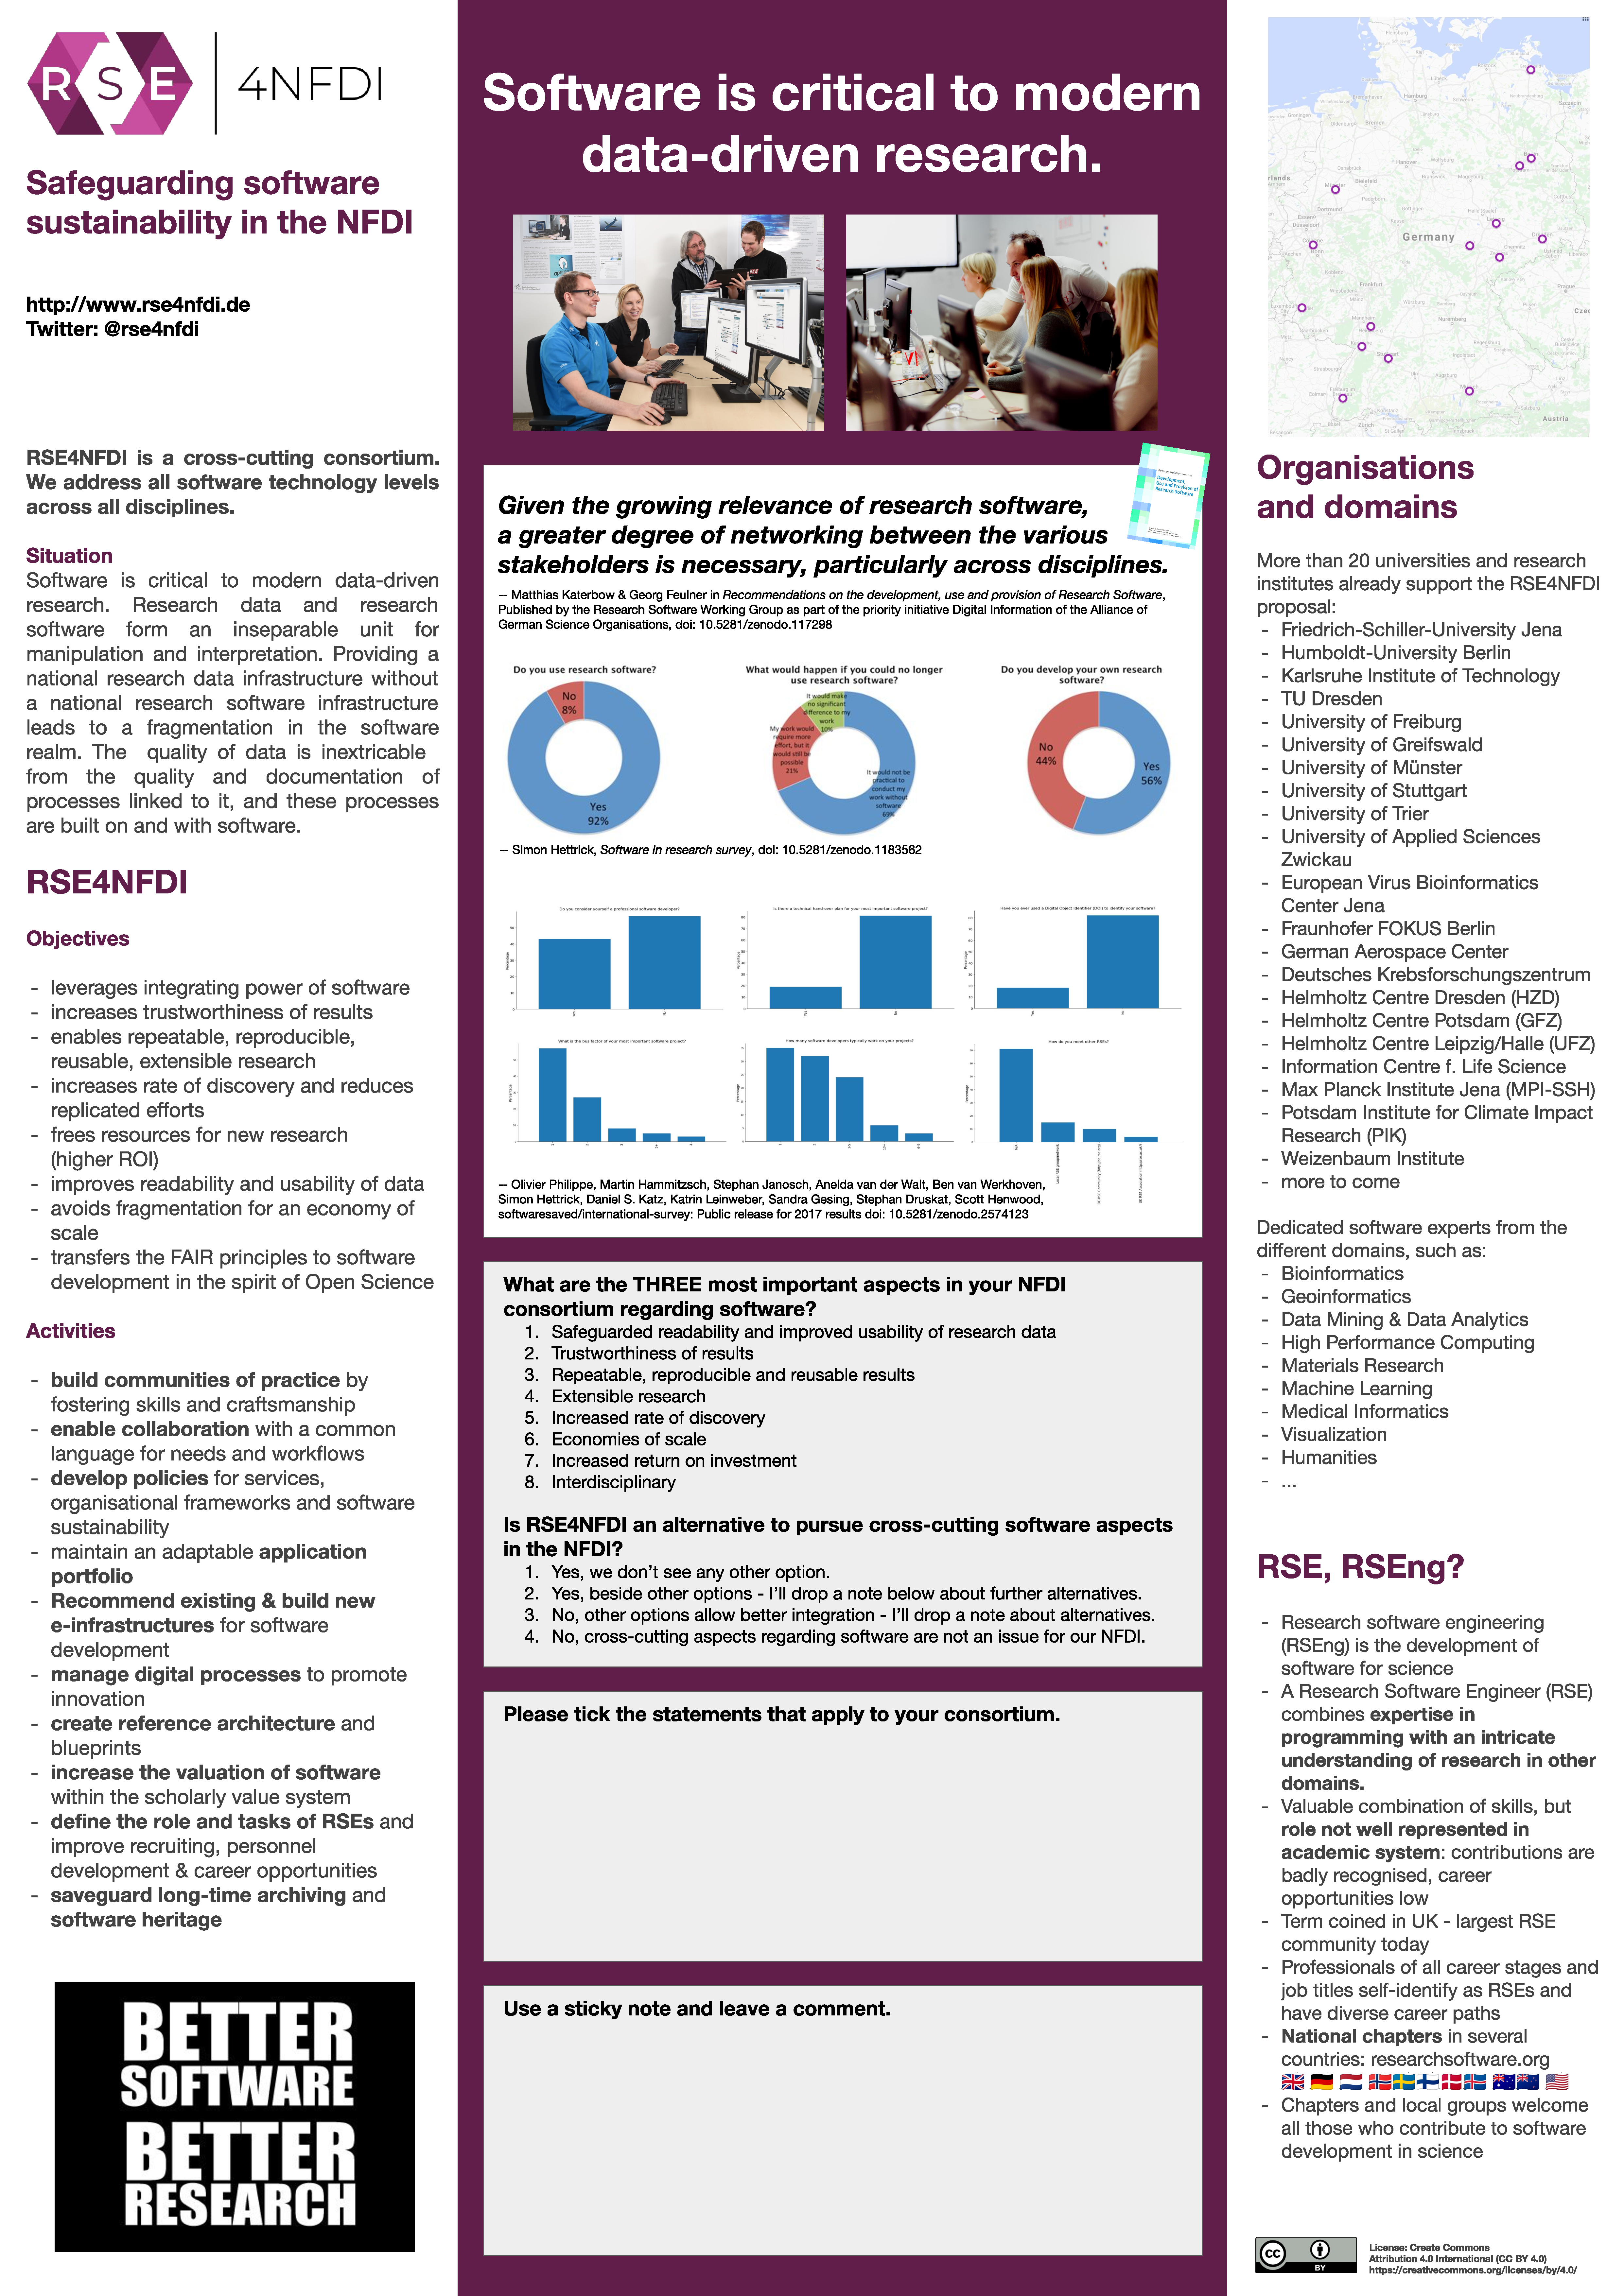
\includegraphics[width=\textwidth]{RSE4NFDI_Poster}\\
 \item \textbf{4.-6.6.}\\
 \textbf{deRSE19} - gemeinsam organisiert mit der Gesellschaft für Informatik e.V. als Hauptveranstalter.\\
 Wir danken den Sponsoren: Microsoft Deutschland GmbH, Amazon Web Services, GitLab, dem R Consortium und dem Python Software Verband e.V.
\end{itemize}

\section{Weitere Ereignisse}

\begin{itemize}
 \item \textbf{Blog}
 \begin{itemize}
  \item \href{https://www.de-rse.org/blog/2019/01/29/umfrageverteilung-2018-in-deutschland.html}{Umfrageverteilung 2018 in Deutschland}
  \item \href{https://www.de-rse.org/blog/2019/02/26/new-rse-groups-meet-in-munich-and-muenster.html}{Neue RSE-Gruppen in München und Münster}
 \end{itemize}
 \item \textbf{Vorstandssitzungen}\\
  Vorstandssitzungen fanden an den folgenden Tagen statt: 7.1., 21.1., 1.2., 19.2., 11.3., 28.3., 17.5. und am 28.5. Alle Sitzungen waren Beschlussfähig. Protokolle sind größtenteils öffentlich unter https://github.com/DE-RSE/protokolle/ einsehbar (laut Beschluss vom 7.1.).
% \item \textbf{wann}\\
%  Vorstellungen von de-RSE auf Veranstaltungen
\end{itemize}

% Mindestinhalt laut https://www.vereinswelt.de/rechenschaftsbericht
%Mitgliederentwicklung: Zu- und Abgang von Mitgliedern, Erläuterungen zu auffälligen Entwicklungen, Ausschlussverfahren
%Durchgeführte Vereinsveranstaltungen
%Teilnahme an Wettbewerben und Ergebnisse
%Beziehungen zum Dachverband und zu anderen Vereinen
%Stand laufender Projekte
%Struktur des Vereins
%Aktivitäten der Organe und Ausschüsse
%Sonstige Ereignisse, die für den Verein wichtig waren
%Finanzbericht
% Empfohlen
%Beziehungen zu Sponsoren und Spendern
%Aktivitäten zur Gewinnung weiterer Sponsoren und Spender
%Ausgang von für den Verein bedeutsamen Gerichtsverfahren
%Hauptamtliche Mitarbeiter, Veränderungen im Personalbestand
%Geplante Projekte und Aktivitäten


\end{document}
